%
% Chapter 2 - Components and requirements
%

\chapter{Components and requirements}

\section{Requirements analysis}

In order to build this multiplaform application a relational database and a HTTP server must be included
in the backend, which will store and supply information to the mobile and web browser clients.\\

The next subsections identify the requirements for each component.

\subsection{Database}

\subsubsection{Functional requirements}

\begin{itemize}
    \item A model that stores and organizes information from diferent sources - APIs and users;
    \item Unify various types of information from various sources into a single entity, named Submission;
    \item Suggest meals for a given restaurant;
    \item Store user sensitive information;
    \item Provide restaurants around any given geolocation;
    \item Seperate data, labeling which ones should be votable, favorable or reportable;
\end{itemize}

\subsubsection{Non-functional requirements}

\begin{itemize}
    \item Performance when searching nearby restaurants;
    \item Query simplicity;
    \item Database normalization;
\end{itemize}

\subsection{HTTP Server}

\subsubsection{Functional requirements}

\begin{itemize}
    \item Provide endpoints that allow users to view and create nearby restaurants and meals;
    \item Provide users the ability to edit their submissions and vote or report others;
    \item Filter content based on a submission's votes and reports;
\end{itemize}

\subsubsection{Non-functional requirements}

\begin{itemize}
    \item Garantee authentication and password encryption when registering;
    \item Encrypt authenticated users' insulin profiles when inserting them into the database;
\end{itemize}

\subsection{Mobile application}

\subsubsection{Functional requirements}

\begin{itemize}
    \item Communicate with the HTTP server in order to display nearby restaurants and their meals based on current geolocation;
    \item Allow users to create restaurants and meals;
    \item Allow authenticated users to create and remove insulin profiles;
    \item Calculate insulin dosages based on a user's blood glucose, insulin profile and the selected meal;
    \item Allow users to vote, report and add submissions to their personal favorites;
    \item Allow mimimum functionalities for unauthenticated users;
\end{itemize}

\subsubsection{Non-functional requirements}

\begin{itemize}
    \item Allow the user to choose its default measurement units;
    \item Allow user authentication and registering;
\end{itemize}

\subsection{Front web application}

\subsubsection{Functional requirements}

\begin{itemize}
    \item Platform administration tools;
    \item Faulty data management;
    \item User control;
\end{itemize}

\subsubsection{Non-functional requirements}

\begin{itemize}
    \item Responsive and performant UI;
\end{itemize}

\section{Component's structure}

To match previously stated requirements the group conceived a platform following the structure
represented by the next picture:\\

\begin{figure}[H]
    \begin{center}
        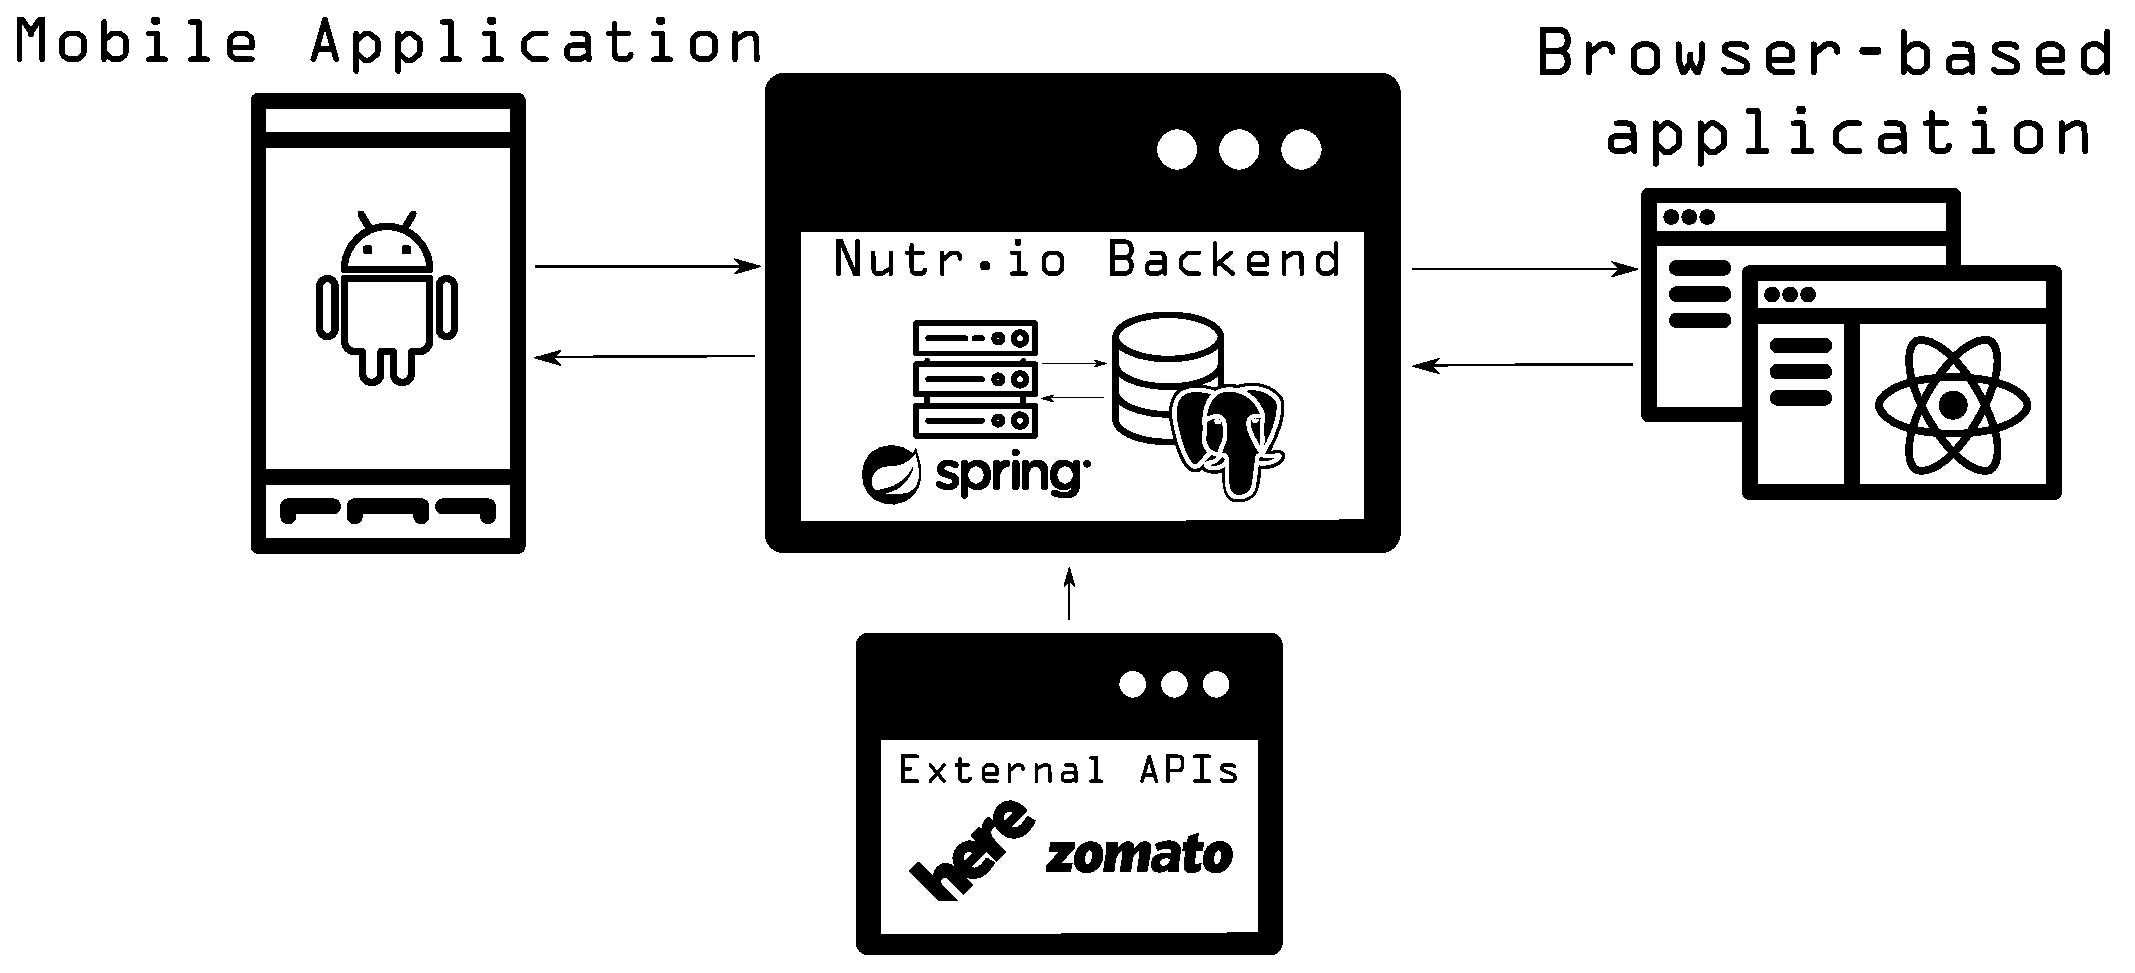
\includegraphics[scale=0.4]{_figures/Nutrio_components.eps}
        \caption{Nutr.io platform components}
    \end{center}
\end{figure}

As shown, the platform will be composed by two clients: a mobile application for Android devices and a web browser
application, which will have as backend a HTTP server and a relational database.\\

External APIs will also be used to obtain restaurants' related information. After some discussion, the group chose
to use the Here API, to provide restaurant information and geolocation.\\

More details about the chosen tecnologies for each component will be described in the fourth chapter of this report.\\

\section{Stakeholders}

Analyzed components and requirements imply the existance of two types of submitters which will interact with the system - an user and external APIs.\\

The way they can interact with the system is as follows:\\

\subsection{User}

An user interacts with the system via a client which can request submissions.
Additionally, if authenticated, an user can create, vote and report submissions; making him the most vital stakeholder when it comes to creating a self-maintained system.

\subsection{External API}

An external API interacts directly with the HTTP server and is resposible in providing nearby restaurants around given geolocation.\\

However, since not all restaurants are registered in utilized APIs, the need for a collaborative user is highly vital when creating a self-maintained system.\\